\section{Celda Universal}

\subsection{Configuraciones correspondientes a distintas celdas universales}

\subsubsection{Kerwin-Huelsman-Newcomb}

\begin{figure}[H] %!ht
	\centering
	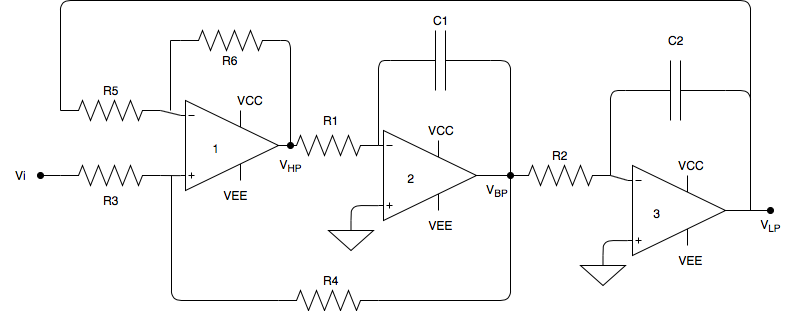
\includegraphics[width=12cm,height=12cm,keepaspectratio]{../EJ4/imagenes/kerwin.png}
	\caption{Circuito Kerwin-Huelsman-Newcomb}
	\label{kerwin}
\end{figure}

\todo{CHEQUEAR circuito porque en el palombo est\'a distinto!}

Dependiendo de d\'onde se tome la salida del circuito \ref{kerwin}, se puede obtener un filtro pasa altos, un pasa banda o un pasabajos. Lo que sucede con Kerwin-Huelsman-Newcomb es que no brinda una salida rechaza banda. La misma puede igual lograrse agregandole al circuito \ref{kerwin} un sumador, como se muestra en la figura \ref{sumador_extra}:

\begin{figure}[H] %!ht
	\centering
	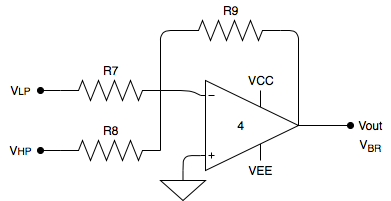
\includegraphics[width=8cm,height=8cm,keepaspectratio]{../EJ4/imagenes/sumador_extra.png}
	\caption{Sumador que se le agrega a la selda para obtener un rechaza banda.}
	\label{sumador_extra}
\end{figure}

\subsubsection{Tow-Thomas}

\begin{figure}[H] %!ht
	\centering
	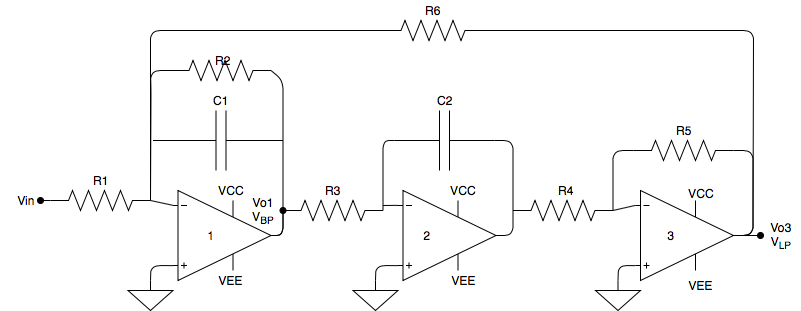
\includegraphics[width=12cm,height=12cm,keepaspectratio]{../EJ4/imagenes/tow_thomas.png}
	\caption{Celda Tow-Thomas}
	\label{tow_thomas}
\end{figure}

La celda Tow-Thomas var\'ia frente a la Kerwin-Huelsman-Newcomb al tener juntos a la entrada el sumador y el primer integrador, agregando luego un inversor y una resistencia en la realimentación que va de la salida $V_{LP}$ a la entrada del circuito. Esta nueva configuraci\'on, al igual que en la Kerwin-Huelsman-Newcomb sigue teniendo una salida de pasa bajos y una de pasa banda, pero ya no tiene una de pasa altos. Esto no importa en nuestro caso al querer obtener un rechaza bandas. Al igual que para el caso anterior, debe agregarse el sumador de la figura \ref{sumador_extra}.

\subsubsection{Ackerberg-Mossberg}

\begin{figure}[H] %!ht
	\centering
	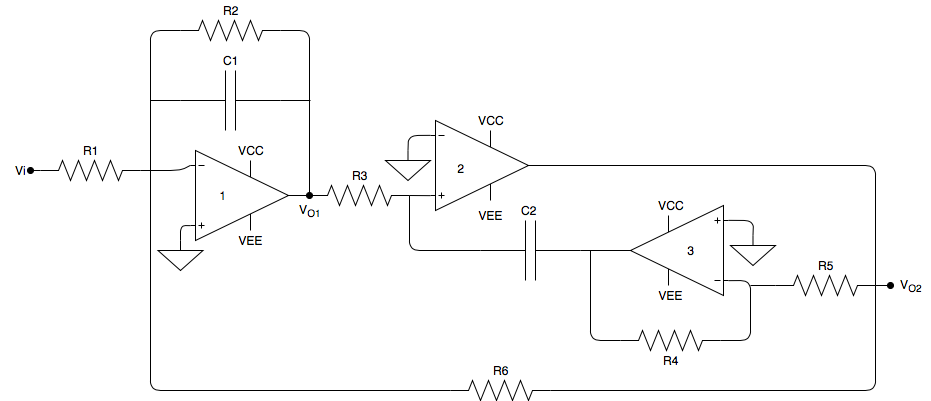
\includegraphics[width=12cm,height=12cm,keepaspectratio]{../EJ4/imagenes/ackerberg.png}
	\caption{Celda Ackerberg-Mossberg}
	\label{ackerberg}
\end{figure}

\subsubsection{Fleischer-Tow}

\begin{figure}[H] %!ht
	\centering
	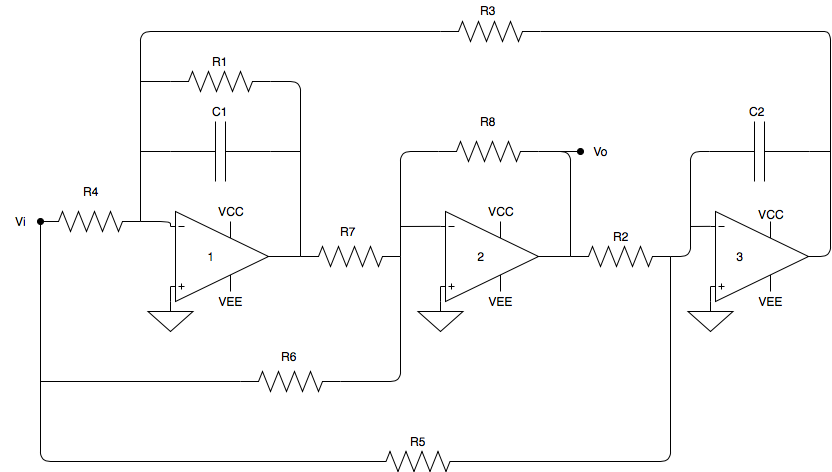
\includegraphics[width=12cm,height=12cm,keepaspectratio]{../EJ4/imagenes/fleischer.png}
	\caption{Celda Fleischer-Tow}
	\label{fleischer}
\end{figure}